\begin{figure}[ht] 
 	\centering 
 	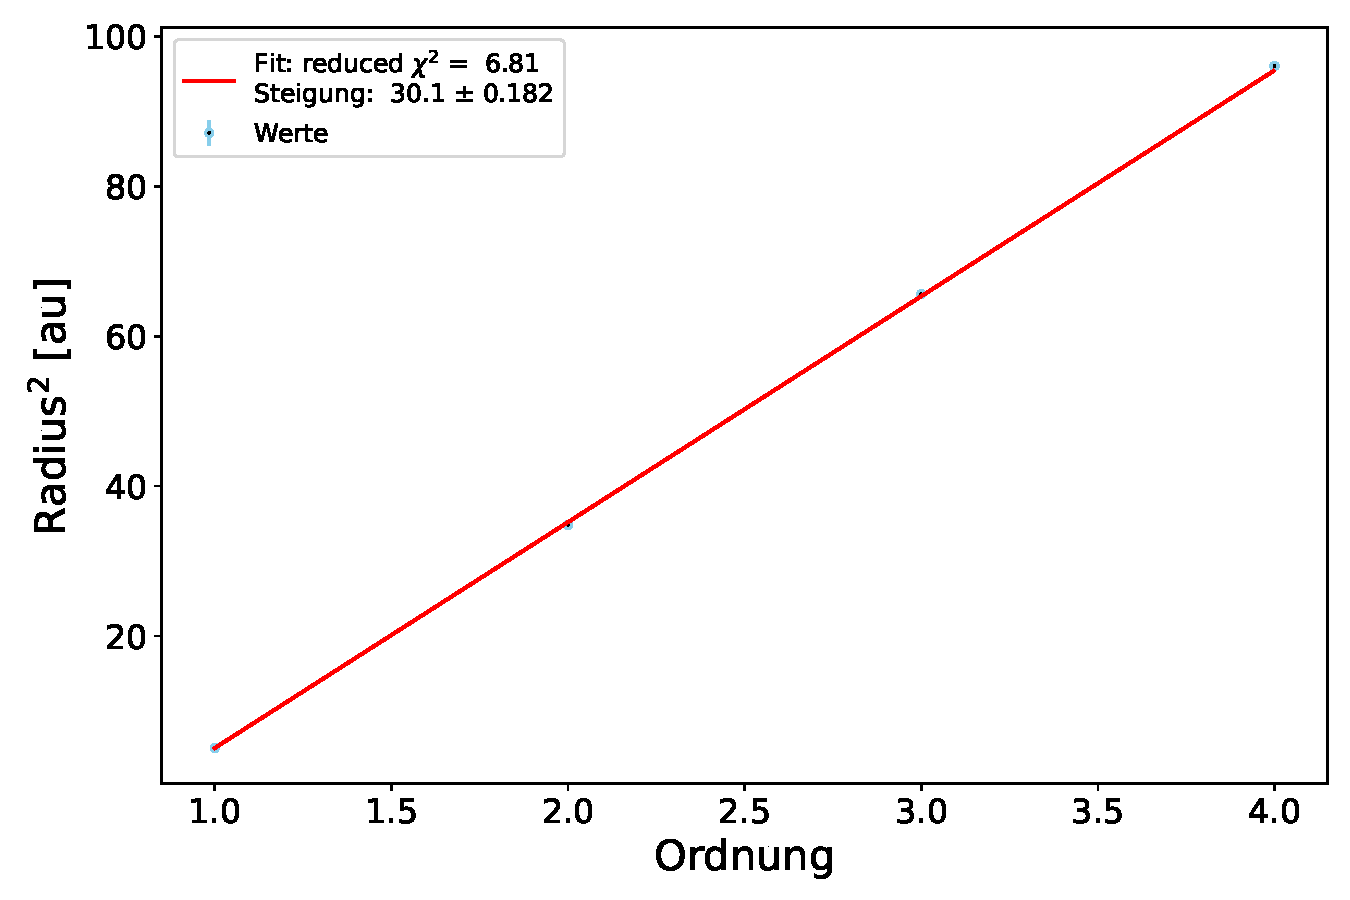
\includegraphics[width= 0.65 \textwidth]{Fits/messung1_Ring2_tim_Fit.pdf} 
	\caption{messung1_Ring2_tim, Fit} 
 	\label{fig:messung1_Ring2_tim, Fit} 
\end{figure}
 \\ 
\begin{table}[ht] 
\centering 
\caption{messung1_Ring1_tim, Fit Parameter Tabelle} 
\label{tab:my-table}
\begin{tabular}{|l|c|}
\hline
Parameter Name	&	Wert \\ \hline
slope	&	 30.136 \pm  0.182\\ \hline
intercept	&	-25.0785 \pm  0.195\\ \hline
\end{tabular} 
\end{table}